\documentclass[a4paper,12pt]{article}
\usepackage[left=2cm,right=2cm, top=2cm,bottom=2cm]{geometry}
\textheight=24cm
\textwidth=16cm
\def\baselinestretch{1.5}
\setlength{\parindent}{5ex}
\linespread {1.5}
\usepackage[utf8]{inputenc}
\usepackage[russian]{babel}
\usepackage[T2A]{fontenc}
\usepackage{amsmath,amsfonts,amssymb,amsthm,mathtools}
\usepackage{indentfirst}
\usepackage{misccorr}
\usepackage{graphicx}
\usepackage{amsmath}
\usepackage{listings}
\pagestyle{empty}
\usepackage{graphics}
\graphicspath{{flowcharts/}}
\DeclareGraphicsExtensions{.png}
\usepackage{color}
\usepackage{xcolor}
\usepackage{hyperref}

\lstset{ %
language=C++,
basicstyle=\small\ttfamily,
stepnumber=1,
numbersep=5pt,
backgroundcolor=\color{white},
showspaces=false,
showstringspaces=false,
showtabs=false,
frame=false,
tabsize=2,
captionpos=t,
breaklines=true,
breakatwhitespace=false,
escapeinside={\%*}{*)},
inputencoding=utf8,
extendedchars=\true
}


\begin{document}
\begin{center}
\large{ФЕДЕРАЛЬНОЕ АГЕНСТВО ПО ОБРАЗОВАНИЮ\\}

\normalsize{Белгородский государственный технологический университет им. В.Г. Шухова}\\
\hfill \break
\normalsize{Кафедра программного обеспечения вычислительной техники и автоматизированных систем}\\
\hfill\break
\hfill \break
\hfill \break
\large{\textbf{Курсовая работа}}\\
\begin{center}
\normalsize{По дисциплине «Основы программирования»}\\
\normalsize{Тема «Решение задачи о поиске прямоугольника наибольшей площади»}
\end{center}
\hfill \break
\hfill \break
\hfill \break
\begin{flushleft}
\normalsize{Автор работы }
\underline{\hspace{2cm}}\hspace{1cm}
Фахретдинов В.С., ВТ — 191\\
\hspace{3cm}
\tiny{ (подпись) \textcolor{white}{\hspace{4.2cm}}}

\end{flushleft}
\begin{flushleft}
\normalsize{Руководитель проекта }
\underline{\hspace{2cm}}\hspace{1cm}
Брусенцева В.С.\\
\hspace{4.5cm}
\tiny{ (подпись) \textcolor{white}{\hspace{4.2cm}}}\\
\begin{flushleft}
\normalsize{Оценка }
\underline{\hspace{3cm}}\hspace{1cm}

\tiny{ (подпись) \textcolor{white}{\hspace{4.2cm}}}

\end{flushleft}

\end{flushleft}
\hfill \break
\hfill \break
\hfill \break

Белгород
2020
\end{center}
\newpage
\thispagestyle{empty} % выключаем отображение номера для этой страницы
\tableofcontents
\newpage

\section*{Введение}
\addcontentsline{toc}{section}{Введение}{
Существует множество различных алгоритмических задач, которые на первый взгляд выглядят не очень применимыми на практике, однако имеют под собой серьёзное обоснование и сложное решение. Одной из таких задач является задача о \textit{максимальном пустом прямоугольнике}(МПП). Её суть состоит в следующем: требуется найти прямоугольник максимального размера, который следует разместить среди препятствий на плоскости~\cite{Naamad}. Задачи этого типа могут возникать при автоматизации проэктирования электроники, в разработке и компоновке интегральных микросхем. Более частным случаем задачи о МПП является другая: допустим, что дан прямоугольник A, содержащий в себе n точек, нужно найти прямоугольник наибольшей площади, стороны которого параллельны прямоугольнику A, лежащий в прямоугольнике A и не содержащий какую-либо из данных точек. Именно один из частных случаев этой задачи и будет рассматриваться в данной работе.
}

\newpage

\section{Постановка задачи курсовой работы}{
Разработка модульной программы на языке C++ для решения следующей задачи. Имеется прямоугольное поле — это участок земли, на котором располагаются прямоугольные здания, параллельные сторонам внешнего участка. Кроме того, на этом участке посажены деревья. Требуется выбрать прямоугольный участок максимальной площади для здания так, чтобы он был построен не ближе чем на метр ко всем препятствиям, а его стороны также располагались параллельно сторонам участка. \\
Введём несколько понятий для данной задачи:\\
$A$ — участок земли, представленный левой нижней точкой $A_{lb}$ и правой верхней точкой $A_{rt}$, каждая точка описывается своими координатами $(X,Y)$. \\$T$ — множество n деревьев, каждое дерево — $T_i, i=1,2,...n,$ также представляет из себя точку, определённую своими координатами.\\ $B$ — множество всех $k$ зданий, каждое здание $B_i$ описывается парой координат нижней левой и правой верхней точек $B_{i_{lb}}, B_{i_{rt}}, i=1,2,...k$,  и каждая из которых в свою очередь также определяется своими координатами.\\
Формат входных данных:\\
Координаты являются целыми числами, один метр равен евклидовому расстоянию между точками $(0,0)$ и $(0,1)$ или же между $(0,0)$ и $(1,0)$.
В первой строке входных данных записано 4 числа — $X$ и $Y$ координаты точек $A_{lb}$ и $A_{rt}$ по очереди, сперва координаты первой, затем второй.\\
Во второй строке записано число $n$, равное количеству деревьев на участке. В следующих $n$ строках идут пары координат $X$ и $Y$ деревьев. \\
В строке после этого записано число $k$, которое определяет количество зданий на участке. И в дальнейших $k$ строках записаны по две пары чисел — $X$ и $Y$ координаты левой нижней и правой верхней точек по очереди, сперва координаты первой, затем второй.\\
Поток ввода — консоль или файл, имя которого вводится в консоль.\\
Формат выходных данных: \\
В строке записаны две пары чисел — $X$ и $Y$ координаты левой нижней и правой верхней точек искомого прямоугольника по очереди, сперва координаты первой, затем второй.\\
Поток вывода — консоль или файл, имя которого вводится в консоль.\\
Кроме того, в результате выполнения программы будет производиться открытие нового окна с графической визуализаций и представлением участка земли в виде белого цвета, деревьев — в виде точек зелёного цвета, зданий — как прямоугольников синего цвета, а искомый МПП будет представлять из себя красный прямоугольник.
}

\newpage

\section{Выбор способа решения задачи} {
\subsection{Переход к задаче о МПП}
Для того, чтобы из данной задачи получить более общую, воспользуемся следующим приёмом. Множество всех точек, которое можно получить из деревьев и зданий, мы переведём в новое множество точек, используя условие того, что наш многоугольник должен распологаться на расстоянии метра от данных препятствий. Для этого построим функцию $f(A, B, T, 1) : \left\{B,T\right\} \rightarrow \left\{S\right\}$. Таким образом, данную задачу мы свели к задаче о МПП, а следовательно, если решим её, то решим и исходную.
\subsection{Решение задачи о МПП}
Простейшим решением, которое лежит на поверхности, является полнопереборный алгоритм. Сперва сформируем множество всех точек, из которых мы можем начать построение нашего многоугольника. Затем, будем по очереди увеличивать наш многоугольник — сперва по диагонали, увеличивая как ширину, так и длину, на каждом шаге проверяя, не входит ли в территорию нашего многоугольника какая-либо точка, и если такая есть, то возвращаемся на шаг назад. Далее, мы будем делать схожее действие, однако увеличивая нашу фигуру сперва в длину, запоминая максимальную площадь и координаты, на которых прервётся данный цикл, если полученная площадь больше, чем сохранённая ранее, а затем в ширину, также запоминая оптимальные параметры. После перебора всех возможных пустых прямоугольников, получим искомое решение. \newline
Несмотря на свою простоту, данное решение не может похвастаться скоростью работы, очевидно, что этот алгоритм крайне неэффективен даже для переборных алгоритмов. Таким образом, следует изменить подход к данной задаче. \newline
Назовём данный \textit{прямоугольник} $P$ \textit{ограниченным} (далее ОП), если для него выполняются условия:
\begin{itemize}
\item Прямоугольник $P$ полностью содержится в прямоугольнике $A$.
\item $P$ не содержит в себе никаких точек.
\item Каждая сторона прямоугольника $P$ либо содержит в себе точку, либо прилегает к стороне прямоугольника $A$.
\end{itemize}
Всего можно выделить 4 типа ОП~\cite{Nandy1}:
\begin{enumerate}
\item В которых противоположные стороны прилегают к сторонам прямоугольника $A$.
\item В которых две смежные стороны прилегают к сторонамм прямоугольника $A$.
\item В которых только одна сторона прилегает к стороне прямоугольника $A$.
\item В которых каждая сторона содержит в себе как минимум одну точку.
\end{enumerate}
Сперва, получив максимальное расстояние $MGAP$ между $x$-овыми координатами всех точек, перемножим его на расстояние между $y$-ковыми координатами верхней и нижней сторон прямоугольника $А$, сохранив это произведение как $MAXR$, а также сохранив соответствующие координаты полученного прямоугольника. Таким образом, данным шагом мы отобрали наибольший МПП среди тех ОП, которые представляют собой тип №1, и в которых сторонами касания являются верхняя и нижняя. \\
Затем, мы отсортируем все точки по $y$-ковым координатам в порядке невозрастания, и будем попарно перебирать каждую пару точек единожды (т.е не учитывая порядок точек в паре). При новом выборе каждой точки мы будем сохранять границы текущего поиска
по $x$ как $T_L$ и $T_R$. Если вторая точка из пары принадлежит данному интервалу, тогда мы посчитаем максимальную площадь прямоугольника, у которого $y$-ковые координаты будут представлять из себя соответствующие координаты выбранных двух точек, а в качестве $x$-овых будут идти $T_L$ и $T_R$. Если полученная площадь больше, чем найденная ранее $MAXR$, сохраним её и искомые координаты. Если вторая точка из выбранной пары больше, чем первая, то сохраним её как левую границу $T_L$, иначе как правую $T_R$. Этими действиями мы определили остальные ОП 1-го типа — стороны которых прилегают в к левым и правым сторонам прямоугольника $A$, ОП типа №2 и №4, а также типа №3, чьи левые или правые стороны прилегают к соответствующим сторонами $A$.  \\
Кроме того, на каждом шаге этого перебора, для каждой точки из первой пары мы посчитаем площадь, беря её $y$-ковую координату и $y$-ковую координату нижней стороны $A$, а в качестве $x$-овых координат будем брать $T_L$ и $T_R$, также сохраняя $MAXR$ и координаты в случае необходимости. Этим мы перебрали ОП типа №3, чья нижняя сторона прилегает к нижней стороне прямоугольника $A$. \\
Нам осталось посчитать только площадь тех ОП типа №3, чья верхняя сторона прилегает к верхней стороне прямоугольника $A$. Для этого мы будем брать каждую точку, находить левую координату $L$, которую будем определять как минимальную среди всех $x$-овых координат точек в обьединении с координатой правой стороны $A$, таких, что её $y$-ковая координата больше выбранной точки, а $x$-овая координата также больше соответствующей координаты выбранной точки. Соответственно, правую координату $R$ мы будем брать как максимальную координату среди всех точек, чья $y$-ковая координата больше координаты этой точки, а $x$-овая координата меньше этой точки. Посчитаем для прямоугольника с $x$-овыми координатами $L$ и $R$, а $y$-ковыми возьмём координату верхней стороны прямоугольника $A$ и $y$-ковую координату для выбранной точки. В очередной раз сохраняем координаты и $MAXR$, если оно получилось максимальным. \\
Теперь мы точно можем сказать, что задача о МПП может быть решена с помощью алгоритма, чья временная сложность оценивается как $O(n^2)$, где $n$ — число точек в прямоугольнике~\cite{Nandy2}.\\
}

\newpage

\section{Выбор структур данных} {
Для решения задачи воспользуемся следующими структурами данных:
\begin{itemize}
\item Point — данная структура представляет из себя простейшую СД, на основе которой будут строиться все дальнейшие СД. Она состоит из двух чисел, которые характеризуют $x$ и $y$ координаты точки. \\
\begin{lstlisting}
struct point {
	int x;
	int y;
};

\end{lstlisting}
\item Rectangle — эта СД служит представлением для прямоугольника. В ней хранятся левая нижняя и правая верхня вершины прямоугольника. \\
\begin{lstlisting}
struct rectangle {
	point lb;
	point rt;
};
\end{lstlisting}
\item Следущая структура, input\_data, представляет из себя набор входных данных для данной задачи. То есть, в ней содержится представление участка земли, в виде прямоугольника, массива деревьев, как массива точек, и массива зданий как массива прямоугольников.\\
\begin{lstlisting}
struct  input_data {
	rectangle A;
	std::vector<point> T;
	std::vector<rectangle> B;
};
\end{lstlisting}
\item Последняя СД, которая необходима в данной задаче — входные данные для задачи о МПП, MERdata. В данной структуре хранится внешняя плоскость в форме прямоугольника, а также массив всех точек.
\begin{lstlisting}
struct MERdata {
	rectangle A;
	std::vector<point> S;
};
\end{lstlisting}
\end{itemize}
}

\newpage

\section{Блок-схема основного алгоритма в укрупнённых блоках} {
\begin{figure}[h!]
\center{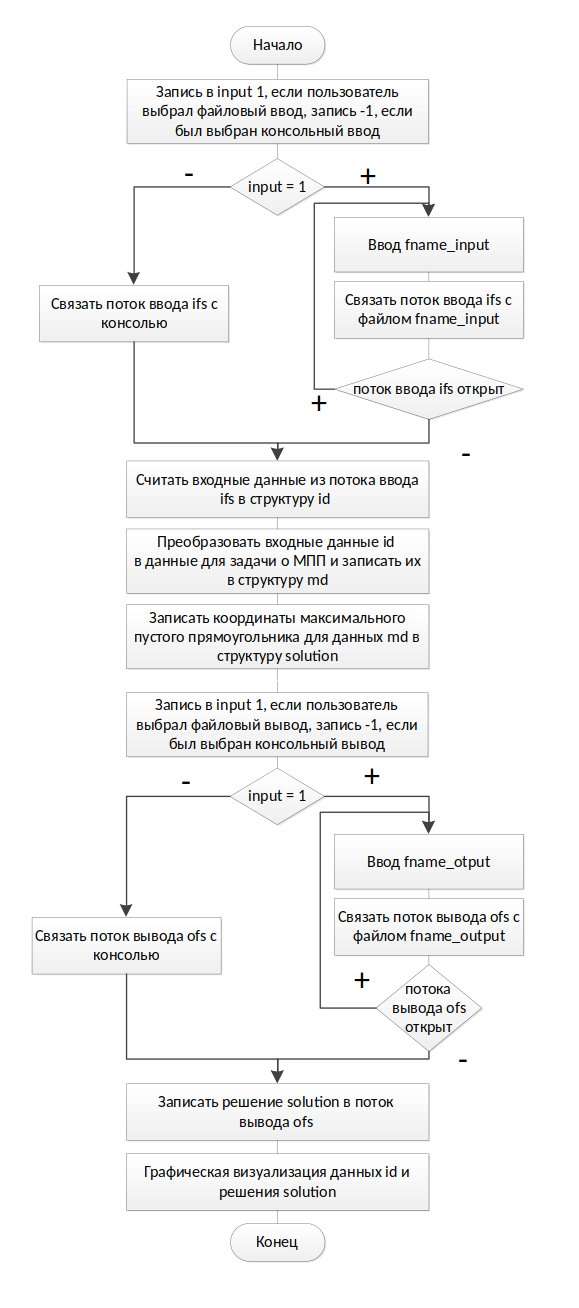
\includegraphics[scale=0.42]{mainalgo.png}}
	{\\Рисунок 1 — Блок-схема в укрупнённых блоках}
\end{figure}

\newpage 

\section{Описание методов} {
\begin{center}
Reader
\end{center}
\begin{itemize}
\item Заголовок: Reader(std::istream\& input\_stream); \\
Назначение: конструктор, инициализация объекта класса Reader, запись потока ввода std::istream\& input\_stream в атрибут класса std::istream\& is.
\item Заголовок: input\_data read\_input\_data(); \\
Назначение: публичный метод, интерфейс для класса, возвращает введёную информацию типа input\_data из потока ввода.
\item Заголовок: input\_data read(); 
Назначение: частный метод, возвращает введёную информацию типа input\_data из потока ввода, сохранённого в атрибуте класса std::istream\& is.
\end{itemize}


\begin{center}
Writer
\end{center}
\begin{itemize}
\item Заголовок: Writer(std::ostream\& output\_stream); \\
Назначение: конструктор, инициализация объекта класса Writer, запись потока вывода std::ostream\& outputs\_stream в атрибут класса std::ostream\& os.
\item Заголовок: void write\_output\_data(rectangle MER); \\
Назначение: публичный метод, записывает в поток вывода координаты прямоугольника rectangle MER.
\item Заголовок: void write(rectangle MER); \\
Назначение: частный метод, записывает в поток вывода, сохранённый в атрибуте класса std::ostream\& os, координаты прямоугольника rectangle MER.
\end{itemize}

\begin{center}
Converter
\end{center}
\begin{itemize}
\item Заголовок: Converter(); \\
Назначение: конструктор, инициализация объекта класса Converter.
\item Заголовок: MERdata convert(input\_data d, int dist);\\
Назначение: частный метод, возвращает информацию MERdata для задачи о МПП, преобразовывая в неё информацию input\_data о задаче поиска прямоугольника максимальной площади отдалённого от всеx обьектов на расстояние dist.
\item Заголовок: MERdata get\_converted\_data(input\_data d, int dist); \\
Назначение: публичный метод, интерфейс для класса, возвращает информацию MERdata для задачи о МПП, преобразовывая в неё информацию input\_data о задаче поиска прямоугольника максимальной площади отдалённого от всеx обьектов на расстояние dist.
\end{itemize}

\begin{center}
MERSolver
\end{center}
\begin{itemize}
\item Заголовок: MERSolver(); \\
Назначение: конструктор, инициализация объекта класса MERSolver.
\item Заголовок: rectangle solve(MERdata md);\\
Назначение: частный метод, возвращает координаты МПП rectangle, для данных MERdata md.
\newpage
\begin{figure}[h!]
\center{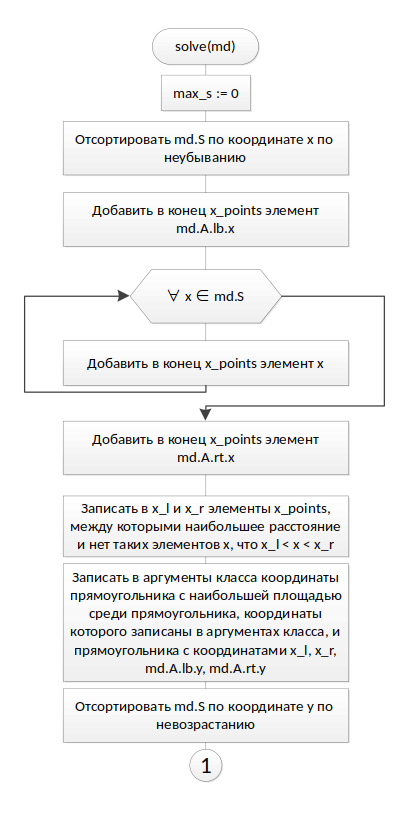
\includegraphics[scale=0.7]{solve1.png}}
	{\\Рисунок 2 — solve, ч1}
\end{figure}
\newpage 
\begin{figure}[h!]
\center{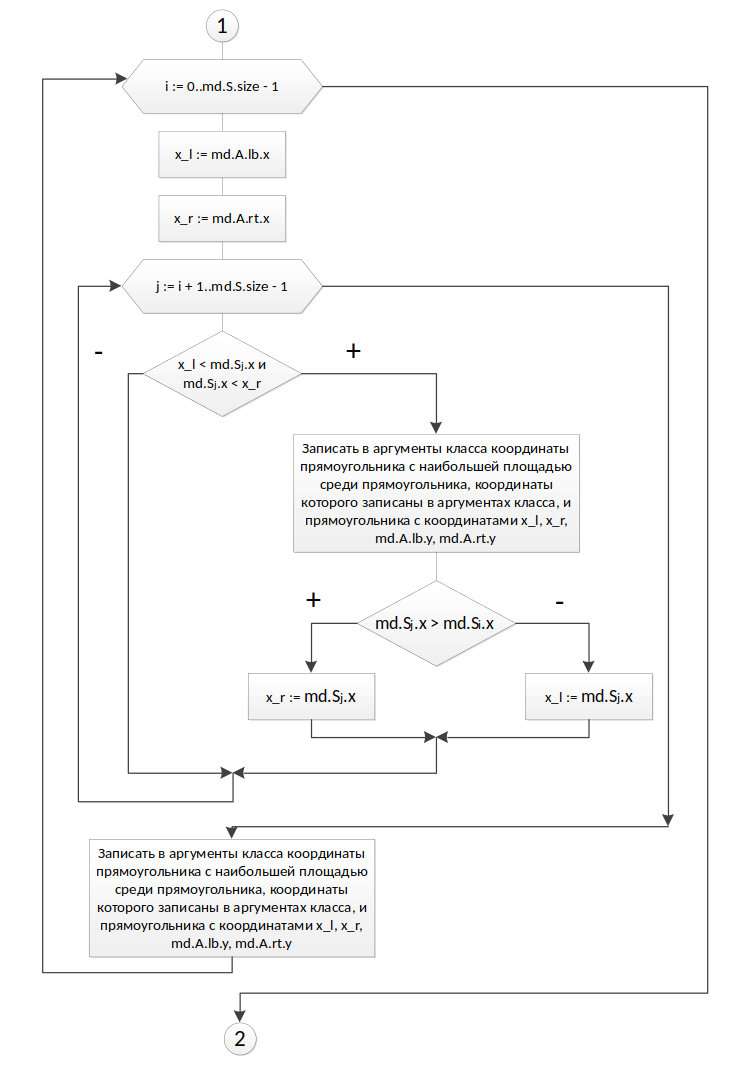
\includegraphics[scale=0.55]{solve2.png}}
	{\\Рисунок 3 — solve, ч2}
\end{figure}
\newpage 
\begin{figure}[h!]
\center{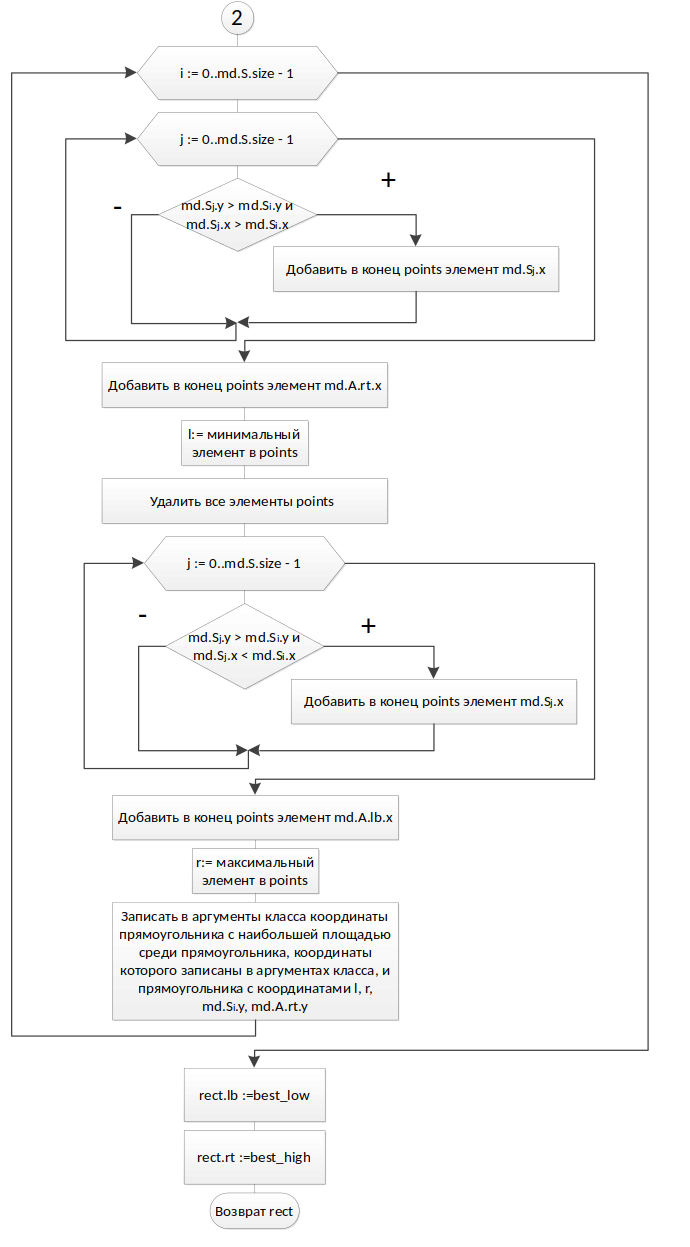
\includegraphics[scale=0.5]{solve3.png}}
	{\\Рисунок 4 — solve, ч3}
\end{figure}
\newpage 
\item Заголовок: void MGAP(std::vector<int> arr, int* left\_best, int* right\_best)\\
Назначение: частный метод, записывает по адресу left\_best и right\_best координаты, между которыми наибольшее расстояние, и нет таких элементов $x$, что left\_best < x < right\_best. 
\item Заголовок: void sort\_by\_coord(std::vector<point>\& arr, bool x, bool asc); \\
Назначение: частный метод, сортирует массив точек std::vector<point> arr по координате $x$, если x является истиной, иначе сортирует по координате $y$, по неубыванию, если $asc$ является истиной, иначе по невозрастанию.
\item Заголовок: void save\_best\_params(int x\_left\_best, int x\_right\_best, int y\_bottom\_best, int y\_top\_best);\\
Назначение: частный метод, записывает в атрибуты класса точки best\_low, best\_high и максимальную площадь max\_s координаты x\_left\_best, x\_right\_best, y\_bottom\_best, y\_top\_best и их площадь, если она больше той, которая записана в max\_s.
\item Заголовок: rectangle get\_solution(MERdata md);\\
Назначение: публичный метод, интерфейс класса, возвращает координаты МПП rectangle, для данных MERdata md.
\end{itemize}

\begin{center}
Render
\end{center}
\begin{itemize}
\item Заголовок: Render(rectangle l\_button, rectangle r\_button);; \\
Назначение: конструктор, инициализация объекта класса Render(), инициализация атрибутов класса rectangle l\_b и r\_b  структурами l\_button и r\_button соответственно.
\item Заголовок: void init();\\
Назначение: частный метод, инициализирует атрибут класса sf::Font font фоном из файла "font.ttf".;
\item Заголовок: void buttons(std::string s, sf::RenderWindow\& w);\\
Назначение: частный метод, вывод в окне w строки s, а также кнопок с координатами, которые хранятся в l\_button и r\_button, и строк FILE и CONSOLE на них. 
\item Заголовок: void solution(input\_data d, rectangle solution, sf::RenderWindow\& w); \\
Назначение: публичный метод, отрисовывает решение задачи с информацией input\_data d о поиске прямоугольника с максимальной площадью с координатами rectangle solution в окне w.
\end{itemize}

\begin{center}
Controller
\end{center}
\begin{itemize}
\item Заголовок: Controller(); \\
Назначение: конструктор, инициализация объекта класса Controller.
\item Заголовок: void run(); \\
Назначение: публичный метод, считавает данные из выбранного потока ввода, решает задачу о поиске прямоугольника с максимальной площадью, удалённого от всех объектов — деревьев, зданий, на 1 метр, записывает решение в выбранный поток вывода, визуализирует решение графически в окне.
\end{itemize}
}

\newpage

\section{Тестовые данные} {
\begin{tabular}{ | l | l | }
\hline
Исходные данные $\hspace{5cm}$ & Результат  $\hspace{5cm}$ \\ \hline
0 0 6 6 & 0 0 2 6  \\ 
2 &     \\ 
5 2 &     \\
4 1 &     \\
1 &     \\
3 3 6 6 &     \\ \hline

0 0 100 100 & 8 0 79 100 \\
3 &     \\
1 1 &     \\
5 5 &     \\
7 7 &     \\
1 &     \\
80 80 100 100 &      \\ \hline

0 0 10 20 & 2 0 6 20 \\
3 &     \\
1 1 &     \\
9 16 &     \\
7 7 &     \\
1 &     \\
8 10 9 14 &     \\ \hline
\end{tabular}
}

\newpage

\section{Разбиение на модули} {
Данную задачу можно разбить на несколько классов:
\begin{enumerate}
\item Reader — класс, отвечающий за считывание входных данных. 
\item Writer — класс, отвечающий за вывод выходных данных.
\item Класс Converter предназначен для преобразования данных исходной задачи в данные задачи о МПП. 
\item MERSolver представляет собой класс, который получает данные и решает задачу о МПП, в результате чего формируются выходные данные.
\item Render — класс, отвечающий за графическую визуализацию.
\item И последний класс, Controller, является управляющим классом. Он взаимодействует с пользователем, управляя классом для визуализации Render и получая режим ввода входных данных и режима вывода выходных, имена файлов для ввода и вывода, если были выбраны соответствующие опции, получает входные данные от класса Reader, передаёт их в Converter. Новые, преобразованные данные, он передаёт классу MERSolver, полученный результат, являющийся решением, Controller отдаёт в класс Writer, а затем заставляет класс Render отобразить исходную задачу в окне приложения.
\end{enumerate}

\newpage

\section*{Заключение}
\addcontentsline{toc}{section}{Заключение}{
В результате данной курсовой работы была решена задача о поиске прямоугольника максимальной площади, удалённого от зданий и деревьев на плоскости. В процессе решения задачи было рассмотрено и проанализировано несколько алгоритмов, из которых был выбран и описан один. \\
Для реализации данного алгоритма была написана модульная программа на языке C++, при написании которой была изучена мультимедийная библиотека SFML~\cite{Link1} для графической визуализации задачи и наглядного представления решения, а также процесс создания архитектуры модульного приложения~\cite{CC}. \\
Мне было интересно решать данную задачу, так как, во-первых, полгода назад я уже видел похожее условие: имелась доска объявлений размером $W \cdot H$, и необходимо было повесить на неё объявление заданной ширины $a$ и неизвестной высоты $b$ так, чтобы площадь пересечения с другими объявлениями была нулевой, и при этом параметр $b$ был бы максимальным.\\
Тогда я не смог её решить из-за нехватки времени, однако теперь я уверен, что на основе данной курсовой работы смогу её решить за отведённое время. А во-вторых, мне принесли удовольствие чтение англоязычных статей, попытки разобраться в терминах и алгоритмах, написание и проектирование архитектуры. С уверенностью могу сказать, что время за работой над курсовой не прошло впустую для меня.
}

\newpage 

\begin{thebibliography}{6}
\addcontentsline{toc}{section}{\bibname}
\bibitem{Naamad}  A. Naamad, D.T. Lee and W.L. Hau, On the maximum empty rectangle problem, Discrete Applied Mathematics 8, 267-277, (1984).
\bibitem{Nandy1} S.C. Nandy and B.B. Bhattachary, Maximal Empty Cuboids
Among Points and Blocks, Computers Math. Applic. Vol. 36, No. 3, pp. 11-20, 1998.
\bibitem{Nandy2} S.C. Nandy and B.B. Bhattachary, On finding an empty staircase polygon of largest area (width)
in a planar point-set, Computational Geometry 26 (2003) 143–171.
\bibitem{Cormen} Томас Х. Кормен, Чарльз И. Лейзерсон, Рональд Л. Ривест, Клиффорд Штайн. Алгоритмы: построение и анализ, 3-е издание = Introduction to Algorithms, Third Edition. — М.: «Вильямс», 2013. — 1328 с.
\bibitem{Link1} URL: \href{https://habr.com/ru/post/480710/}{Рефакторинг игры на SFML}
\bibitem{CC} Макконнелл С., Совершенный код. Мастер-класс / Пер. с англ. — М. : Издательство «Русская
редакция», 2010. — 896 стр. : ил.
\end{thebibliography}

\newpage

\section*{Приложение}
\addcontentsline{toc}{section}{Приложение}{
\begin{center}
"Types.h"
\end{center}
\begin{lstlisting}
#pragma once
#include <iostream>
#include <vector>

static const int WINDOW_SIZE = 600;

struct point {

	int x;
	int y;

};

struct rectangle {

	point lb;
	point rt;

};

struct  input_data {

	rectangle A;
	std::vector<point> T;
	std::vector<rectangle> B;

};

struct MERdata {

	rectangle A;
	std::vector<point> S;

};
\end{lstlisting}
\newpage
\begin{center}
"Reader.h"
\end{center}
\begin{lstlisting}
#pragma once
#include <iostream>
#include "Types.h"

class Reader {

private:

	std::istream& is;
	input_data read();

public:

	Reader(std::istream& input_stream);
	input_data read_input_data();

};
\end{lstlisting}
\newpage
\begin{center}
"Reader.cpp"
\end{center}
\begin{lstlisting}
#include "Reader.h"
#define CATCH_CONFIG_MAIN
#include <iostream>

Reader::Reader(std::istream& input_stream) : is(input_stream) {

}

input_data Reader::read() {

	input_data d;
	is >> d.A.lb.x;
	is >> d.A.lb.y;
	is >> d.A.rt.x;
	is >> d.A.rt.y;

	int n;
	is >> n;
	d.T.resize(n);

	for (int i = 0; i < n; i++) {
		
		is >> d.T[i].x;
		is >> d.T[i].y;

	}

	int k;
	is >> k;
	d.B.resize(k);

	for (int i = 0; i < k; i++) {

		is >> d.B[i].lb.x;
		is >> d.B[i].lb.y;
		is >> d.B[i].rt.x;
		is >> d.B[i].rt.y;

	}

	return d;

}

input_data Reader::read_input_data() {

		return read();

}
\end{lstlisting}
\newpage
\begin{center}
"Writer.h"
\end{center}
\begin{lstlisting}
#pragma once
#include <iostream>
#include "Types.h"

class Writer
{

private:

	std::ostream& os;
	void write(rectangle MER);

public:

	Writer(std::ostream& output_stream);
	void write_output_data(rectangle MER);

};
\end{lstlisting}
\newpage
\begin{center}
"Writer.cpp"
\end{center}
\begin{lstlisting}
#include "Writer.h"

void Writer::write(rectangle MER) {

	os << MER.lb.x << " ";
	os << MER.lb.y << " ";
	os << MER.rt.x << " ";
	os << MER.rt.y << " " << std::endl;

}

Writer::Writer(std::ostream& output_stream): os(output_stream) {


}

void Writer::write_output_data(rectangle MER) {

	write(MER);

}
\end{lstlisting}
\newpage
\begin{center}
"Render.h"
\end{center}
\begin{lstlisting}
#pragma once
#include "Types.h"
#include <SFML/Graphics.hpp>

class Render
{

	sf::Font font;
	void init();
	rectangle l_b;
	rectangle r_b;
	

public:

	Render(rectangle l_button, rectangle r_button);
	void buttons(std::string s, sf::RenderWindow& w);
	void solution(input_data d, rectangle solution, sf::RenderWindow& w);

};
\end{lstlisting}
\newpage
\begin{center}
"Render.cpp"
\end{center}
\begin{lstlisting}
#include "Render.h"

void Render::init() {

	if (!font.loadFromFile("font.ttf")) throw;

}

Render::Render(rectangle l_button, rectangle r_button) {

	l_b = l_button;
	r_b = r_button;
	init();

}

void Render::buttons(std::string s, sf::RenderWindow& w) {

	w.clear();
	sf::RectangleShape shape(sf::Vector2f(l_b.rt.x - l_b.lb.x, l_b.rt.y - l_b.lb.y ));
	shape.setOutlineThickness(2.f);
	shape.setFillColor(sf::Color::Transparent);
	shape.setOutlineColor(sf::Color::Red);
	shape.setPosition(l_b.lb.x, l_b.lb.y);
	w.draw(shape);
	shape.setSize(sf::Vector2f(r_b.rt.x - r_b.lb.x, r_b.rt.y - r_b.lb.y));
	shape.setPosition(r_b.lb.x, r_b.lb.y);
	w.draw(shape);
	sf::Text text("FILE", font);
	text.setPosition(l_b.lb.x, l_b.lb.y);
	text.setCharacterSize(30);
	text.setStyle(sf::Text::Bold);
	text.setFillColor(sf::Color::Red);
	w.draw(text);
	text.setString("CONSOLE");
	text.setPosition(r_b.lb.x, r_b.lb.y);
	w.draw(text);
	text.setString(s);
	text.setPosition(0,0);
	w.draw(text);
	w.display();

}

void Render::solution(input_data d, rectangle solution, sf::RenderWindow& w) {

	w.clear();
	int shape_size = (d.A.rt.x - d.A.lb.x) > (d.A.rt.y - d.A.lb.y) ? (d.A.rt.x - d.A.lb.x) : (d.A.rt.y - d.A.lb.y);
	shape_size = WINDOW_SIZE / shape_size;

	sf::RectangleShape shape(sf::Vector2f((d.A.rt.x - d.A.lb.x) * shape_size, (d.A.rt.y - d.A.lb.y) * shape_size));
	shape.setPosition(0, 0);
	shape.setFillColor(sf::Color::White);
	w.draw(shape);
	
	shape.setSize(sf::Vector2f((solution.rt.x - solution.lb.x) * shape_size, (solution.rt.y - solution.lb.y) * shape_size));
	shape.setPosition(solution.lb.x * shape_size, WINDOW_SIZE - solution.rt.y * shape_size);
	shape.setOutlineColor(sf::Color::White);
	shape.setOutlineThickness(1.f);
	shape.setFillColor(sf::Color::Red);
	w.draw(shape);
	
	sf::CircleShape circle(shape_size/4);
	circle.setFillColor(sf::Color::Green);
	circle.setOutlineColor(sf::Color::White);
	circle.setOutlineThickness(1.f);
	for (auto p : d.T) {

		circle.setPosition(sf::Vector2f((p.x * shape_size) - shape_size/4, WINDOW_SIZE - p.y * shape_size - shape_size/4));
		w.draw(circle);

	}

	shape.setFillColor(sf::Color::Blue);
	for (auto b : d.B) {

		shape.setSize(sf::Vector2f((b.rt.x - b.lb.x) * shape_size, (b.rt.y - b.lb.y) * shape_size));
		shape.setPosition(b.lb.x * shape_size, WINDOW_SIZE - b.rt.y * shape_size);
		w.draw(shape);

	}

	w.display();

}
\end{lstlisting}
\newpage
\begin{center}
"Converter.h"
\end{center}
\begin{lstlisting}
#pragma once
#include "Types.h"

class Converter {

private:

	MERdata convert(input_data d, int dist);

public:

	Converter();
	MERdata get_converted_data(input_data d, int dist);
	
};
\end{lstlisting}
\newpage
\begin{center}
"Converter.cpp"
\end{center}
\begin{lstlisting}
#include "Converter.h"

MERdata Converter::convert(input_data d, int dist) {

	MERdata md;
	md.A.lb = d.A.lb;
	md.A.rt = d.A.rt;

	bool l = true, r = true, t = true, b = true;

	for (auto p : d.T) {

		if (p.x == d.A.lb.x) {

			l = false;

		}

		else if (p.x == d.A.rt.x) {

			r = false;

		}

		if (p.y == d.A.lb.y) {

			b = false;

		}

		else if (p.y == d.A.rt.y) {

			t = false;

		}

		if (l) {

			md.S.push_back({ p.x - dist, p.y });
			if (t) {

				md.S.push_back({ p.x - dist, p.y + dist });

			}

			if (b) {

				md.S.push_back({ p.x - dist, p.y - dist });

			}


		}

		if (t) {

			md.S.push_back({ p.x, p.y + dist });

		}

		if (b) {

			md.S.push_back({ p.x, p.y - dist });

		}

		if (r) {

			md.S.push_back({ p.x + dist, p.y });
			if (t) {

				md.S.push_back({ p.x + dist, p.y + dist });

			}

			if (b) {

				md.S.push_back({ p.x + dist, p.y - dist });

			}

		}

		l = true, r = true, t = true, b = true;

	}

	for (auto rect : d.B) {

		if (rect.lb.x == d.A.lb.x) {

			l = false;

		}

		else if (rect.rt.x == d.A.rt.x) {

			r = false;

		}

		if (rect.lb.y == d.A.lb.y) {

			b = false;

		}

		else if (rect.rt.y == d.A.rt.y) {

			t = false;

		}

		if (l) {

			int diff = rect.rt.y - rect.lb.y;

			for (int y = 0; y <= diff; y++) {

				md.S.push_back({rect.lb.x - dist, rect.lb.y + y});

			}

			diff = rect.rt.x - rect.lb.x;
			if (t) {

				md.S.push_back({rect.lb.x - dist, rect.rt.y + dist});

			}

			if (b) {

				md.S.push_back({rect.lb.x - dist, rect.lb.y - dist});

			}


		}

		int diff = rect.rt.x - rect.lb.x;
		if (t) {

			for (int x = 0; x <= diff; x++) {

				md.S.push_back({ rect.lb.x + x, rect.rt.y + dist });

			}

		}

		if (b) {

			for (int x = 0; x <= diff; x++) {

				md.S.push_back({ rect.lb.x + x, rect.lb.y - dist });

			}

		}


		if (r) {

			int diff = rect.rt.y - rect.lb.y;

			for (int y = 0; y <= diff; y++) {

				md.S.push_back({rect.rt.x + dist, rect.lb.y + y});

			}

			if (t) {

				md.S.push_back({rect.rt.x + dist, rect.rt.y + dist});

			}

			if (b) {

				md.S.push_back({rect.rt.x + dist, rect.lb.y - dist});

			}

		}

		l = true, r = true, t = true, b = true;

	}

	return md;

}

Converter::Converter() {

}

MERdata Converter::get_converted_data(input_data d, int dist) {

	return convert(d, dist);

}
\end{lstlisting}
\newpage
\begin{center}
"MERSolver.h"
\end{center}
\begin{lstlisting}
#pragma once
#include "Types.h"

class MERSolver
{

private:

	point best_low;
	point best_high;
	int max_s;

	void MGAP(std::vector<int> arr, int* left_best, int* right_best);
	void sort_by_coord(std::vector<point>& arr, bool x, bool asc);
	void save_best_params(int x_left_best, int x_right_best, int y_bottom_best, int y_top_best);
	rectangle solve(MERdata md);

public:

	MERSolver();
	rectangle get_solution(MERdata md);

};
\end{lstlisting}
\newpage
\begin{center}
"MERSolver.cpp"
\end{center}
\begin{lstlisting}
#include "MERSolver.h"
#include <algorithm>

MERSolver::MERSolver() {

}

void MERSolver::save_best_params(int x_left_best, int x_right_best, int y_bottom_best, int y_top_best) {

	int t = (x_right_best - x_left_best) * (y_top_best - y_bottom_best);
	if (t > max_s) {

		// сохраняем лучшие параметры
		best_low.x = x_left_best;
		best_low.y = y_bottom_best;

		best_high.x = x_right_best;
		best_high.y = y_top_best;

		max_s = t;

	}

}

void MERSolver::sort_by_coord(std::vector<point>& arr, bool x, bool asc) {

	int i, j;
	point key;

	int param = 1;
	if (!asc) {
	
		param = -1;

	}

	if (x) {

		for (i = 1; i < arr.size(); i++)
		{

			key = arr[i];
			j = i - 1;

			while (j >= 0 && arr[j].x * param > key.x * param)
			{

				arr[j + 1] = arr[j];
				j = j - 1;

			}
			arr[j + 1] = key;

		}

	}

	else {

		for (i = 1; i < arr.size(); i++)
		{

			key = arr[i];
			j = i - 1;

			while (j >= 0 && arr[j].y * param > key.y * param)
			{

				arr[j + 1] = arr[j];
				j = j - 1;

			}

			arr[j + 1] = key;

		}

	}

}

void MERSolver::MGAP(std::vector<int> arr, int* left_best, int* right_best) {

	int max_gap = 0;
	int t;

	for (int i = 0; i < arr.size() - 1; i++) {

		t = arr[i + 1] - arr[i];
		if (t > max_gap) {

			*left_best = arr[i];
			*right_best = arr[i + 1];
			max_gap = t;

		}

	}

}

rectangle MERSolver::solve(MERdata md) {

	max_s = 0;

	int x_l, x_r;
	sort_by_coord(md.S, true, true);

	std::vector<int> x_points;
	x_points.push_back(md.A.lb.x);
	for (auto p : md.S) {

		x_points.push_back(p.x);

	}
	x_points.push_back(md.A.rt.x);

	MGAP(x_points, &x_l, &x_r);
	save_best_params(x_l, x_r, md.A.lb.y, md.A.rt.y);

	sort_by_coord(md.S, false, false);

	for (int i = 0; i < md.S.size(); i++) {

		x_l = md.A.lb.x;
		x_r = md.A.rt.x;
		
		for (int j = i + 1; j < md.S.size(); j++) {

			if ((x_l < md.S[j].x) and ( md.S[j].x < x_r)) {

				save_best_params(x_l, x_r, md.S[j].y, md.S[i].y);

				if (md.S[j].x > md.S[i].x) {

					x_r = md.S[j].x;

				}

				else {

					x_l = md.S[j].x;

				}

			}

		}

		save_best_params(x_r, x_l, md.A.lb.y, md.S[i].y);

	}

	for (int i = 0; i < md.S.size(); i++) {

		std::vector<int> points;

		for (int j = 0; j < md.S.size(); j++) {

			if ((md.S[j].y > md.S[i].y) and (md.S[j].x > md.S[i].x)) {

				points.push_back(md.S[j].x);

			}

		}

		points.push_back(md.A.rt.x); 

		int l = *std::min_element(points.begin(), points.end());

		points.resize(0);

		for (int j = 0; j < md.S.size(); j++) {

			if ((md.S[j].y > md.S[i].y) and (md.S[j].x < md.S[i].x)) {

				points.push_back(md.S[j].x);

			}

		}

		points.push_back(md.A.lb.x); 

		int r = *std::max_element(points.begin(), points.end());

		save_best_params(l, r,  md.S[i].y, md.A.rt.y);

	}

	return { best_low, best_high };


}
	
rectangle MERSolver::get_solution(MERdata md) {

	return solve(md);

}
\end{lstlisting}
\newpage
\begin{center}
"Controller.h"
\end{center}
\begin{lstlisting}
#pragma once
#include "Converter.h"
#include "MERSolver.h"
#include "Reader.h"
#include "Render.h"
#include "Writer.h"
#include "Types.h"

class Controller
{

public:

	Controller();
	void run();

};
\end{lstlisting}
\newpage
\begin{center}
"Controller.cpp"
\end{center}
\begin{lstlisting}
#include "Controller.h"
#include <SFML/Graphics.hpp>
#include "SFML/System.hpp"
#include <fstream>

// константы для кнопок
static rectangle l_b = { {100, 300}, {180, 340} };
static rectangle r_b = { {350, 300}, {485, 340} };

Controller::Controller() {

}

void Controller::run() {

	sf::Event event;
	Render render(l_b, r_b);

	sf::RenderWindow window(sf::VideoMode(WINDOW_SIZE, WINDOW_SIZE), "MER programm");
	window.setFramerateLimit(60);

	int input = 0;
	while (window.isOpen() && (!input)) {

		render.buttons("INPUT", window);

		while (window.pollEvent(event)) {

			if (event.type == sf::Event::Closed) {

				window.close();

			}

			if (event.type = sf::Event::KeyPressed) {

				if (event.key.code == sf::Keyboard::Escape) window.close();

			}

			if (sf::Mouse::isButtonPressed(sf::Mouse::Left)) {

				sf::Vector2i localPosition =  sf::Mouse::getPosition(window);

				if ((localPosition.x > l_b.lb.x) and (localPosition.x < l_b.rt.x) and (localPosition.y > l_b.lb.y) and (localPosition.y < l_b.rt.y)) {

					input = 1;

				}

				if ((localPosition.x > r_b.lb.x) and (localPosition.x < r_b.rt.x) and (localPosition.y > r_b.lb.y) and (localPosition.y < r_b.rt.y)) {

					input = -1;

				}

			}

		}

	}

	std::string fname_input = "input.txt";
	std::ifstream ifs;
	if (input == 1) {

		ifs.exceptions(std::ifstream::failbit);
		while (!ifs.is_open()) {

			try {

				std::cout << "Введите имя файла с входными данными: ";
				std::getline(std::cin, fname_input);
				ifs.open(fname_input, std::ifstream::out);

			}
			catch (const std::ifstream::failure & e) {

				std::cout << "Невозможно открыть файл, проверьте его имя и попробуйте ещё раз.\n";

			}

		}

	}
	else {

		std::cout << "Введите данные: " << std::endl;

	}

	std::istream& is = input == 1 ? ifs : std::cin;

	Reader reader(is);
	Converter converter;
	MERSolver solver;

	input_data id = reader.read_input_data();
	MERdata md = converter.get_converted_data(id, 1);
	rectangle solution = solver.get_solution(md);

	input = 0;
	while (window.isOpen() && (!input)) {

		render.buttons("OUTPUT", window);

		while (window.pollEvent(event)) {

			if (event.type == sf::Event::Closed) {

				window.close();

			}

			if (event.type = sf::Event::KeyPressed) {

				if (event.key.code == sf::Keyboard::Escape) window.close();

			}

			if (sf::Mouse::isButtonPressed(sf::Mouse::Left)) {

				sf::Vector2i localPosition =  sf::Mouse::getPosition(window);

				if ((localPosition.x > l_b.lb.x) and (localPosition.x < l_b.rt.x) and (localPosition.y > l_b.lb.y) and (localPosition.y < l_b.rt.y)) {

					input = 1;

				}

				if ((localPosition.x > r_b.lb.x) and (localPosition.x < r_b.rt.x) and (localPosition.y > r_b.lb.y) and (localPosition.y < r_b.rt.y)) {

					input = -1;

				}

			}

		}

	}

	std::string fname_output = "output.txt";
	std::ofstream ofs;
	if (input == 1) {

		ofs.exceptions(std::ofstream::failbit);
		while (!ofs.is_open()) {

			try {

				std::cout << "Введите имя файла для вывода: ";
				std::getline(std::cin, fname_output);
				ofs.open(fname_output, std::ofstream::out);

			}
			catch (std::ios_base::failure & fail) {

				std::cout << "Невозможно открыть файл, попробуйте ещё раз.\n";

			}

		}

	}
	else {

		std::cout << "Решение: " << std::endl;

	}
	std::ostream& os = input == 1 ? ofs : std::cout;

	Writer writer(os);
	writer.write_output_data(solution);

	while (window.isOpen()) {

		if (event.type == sf::Event::Closed) {

			window.close();

		}

		if (event.type = sf::Event::KeyPressed) {

			if (event.key.code == sf::Keyboard::Escape) window.close();

		}

		render.solution(id, solution, window);

	}

}
\end{lstlisting}
\newpage
\begin{center}
"Programm.cpp"
\end{center}
\begin{lstlisting}
#include "Controller.h"
#include <locale.h>

int main()
{

	setlocale(LC_ALL, "RUS");
	Controller controller;
	controller.run();
	
}
\end{lstlisting}
}

\end{document}